\chapter{METODOLOGI}
\label{chap:desainimplementasi}

% Ubah bagian-bagian berikut dengan isi dari desain dan implementasi

Metodologi berisi tentang langkah-langkah yang akan dilakukan pada penelitian kali ini. Langkah-langkah tersebut akan digambarkan dengan menggunakan blok diagram. Pada penelitian ini terdapat dua buah blok diagram yang masing-masing blok diagram akan merepresentasikan langkah-langkah untuk \emph{hardware} dan \emph{software}.

\section{\emph{Hardware}}

% Contoh input gambar dengan format *.jpg
\begin{figure} [H] \centering
  % Nama dari file gambar yang diinputkan
  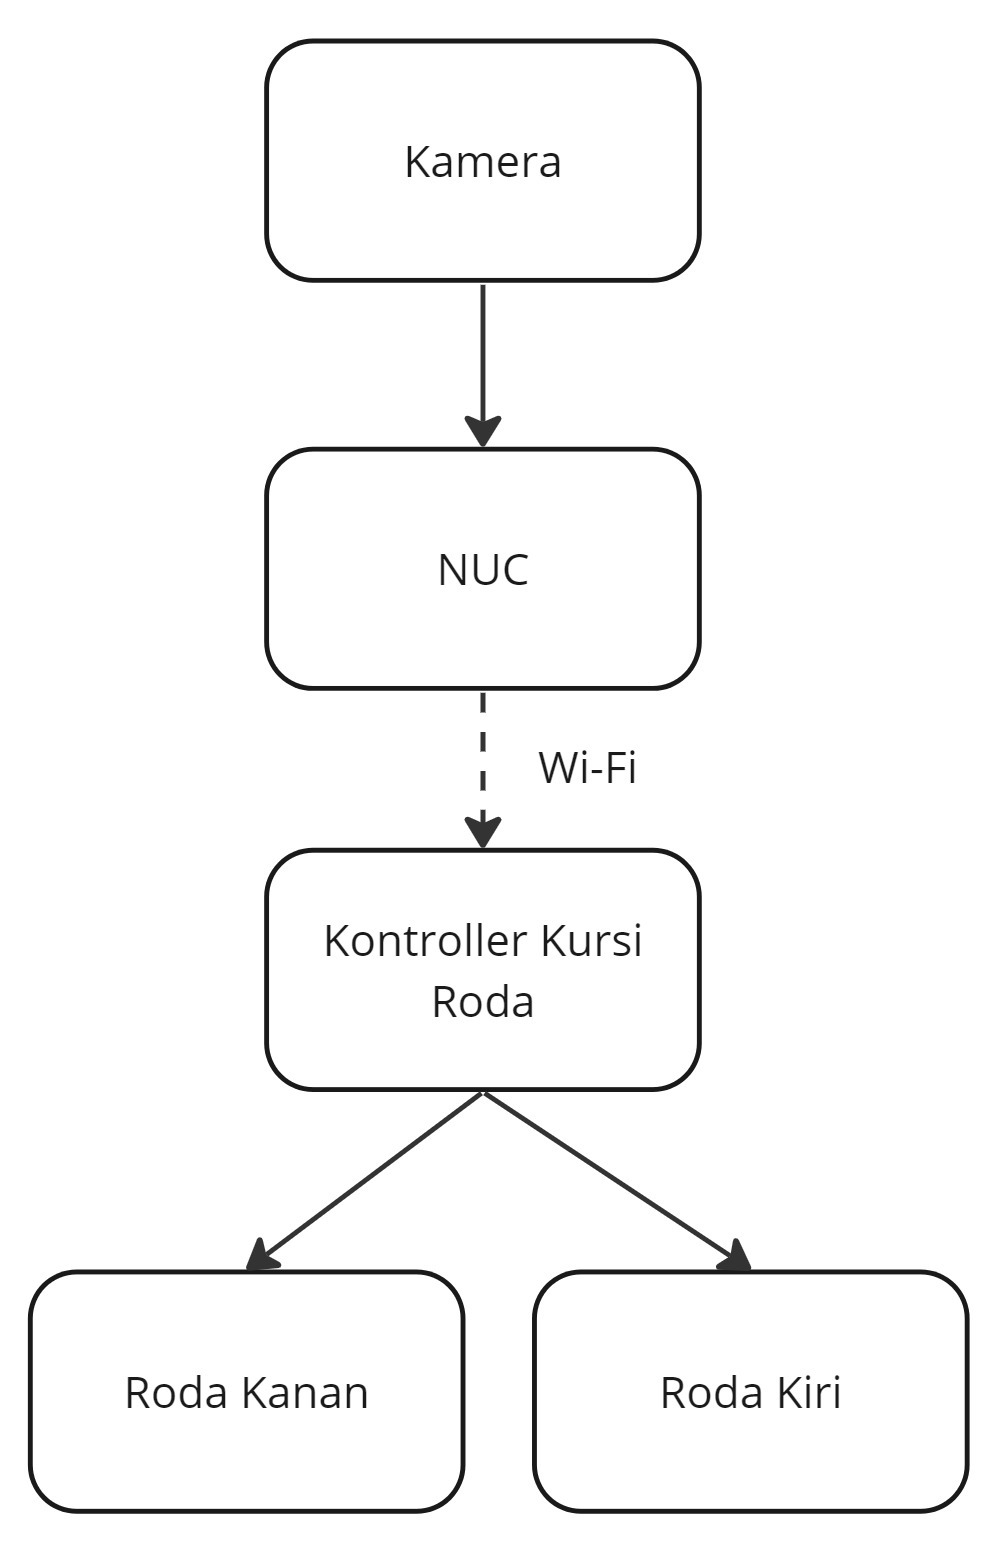
\includegraphics[width=0.6\textwidth]{gambar/blokdiagramidfix.jpg}
  % Keterangan gambar yang diinputkan
  \caption{Blok diagram \emph{hardware}}
  % Label referensi dari gambar yang diinputkan
  \label{fig:Blok Diagram}
\end{figure}

\subsection{NUC}
Pada tahapan ini, dilakukanlah akuisisi data dengan menggunakan kamera yang telah dipasangkan pada bracket yang memungkinkan kamera sejajar dengan wajah pengguna kursi roda. Kemudian, dilakukanlah serangkaian pengolahan data citra wajah oleh mediapipe dan model.h5 yang sudah di-\emph{training} dan berada pada NUC. Setelah itu, hasil klasifikasi yang didapatkan akan dikirimkan oleh NUC ke ESP32 dengan melalui WiFi agar output yang didapatkan bisa desainimplementasikan pada motor kursi roda. Untuk dapat melakukan tahapan tersebut, NUC harus terhubung dengan \emph{access point} ESP32.

Untuk proses pengiriman data hasil pengklasifikasian ke ESP32, telah direpresentasikan pada flowchart Gambar \ref{fig:Flowchart Mengirim Data String Melalui WiFi} sesuai dengan penelitian yang telah dilakukan \parencite{ekatama2024perancangan} dengan judul Perancangan Sistem Kontrol Motor Kursi Roda Secara Nirkabel Berbasis ESP32. Pengiriman ini menggunakan bahasa pemrograman Python dan dirancang untuk mengirim dalam bentuk string. Agar dapat membuat koneksi untuk mengirim dan menerima data melalui jarigan, digunakan beberapa \emph{library} seperti socket, time, dan datetime. Selain itu, IP Address yang dimiliki oleh \emph{Access Point} ESP32 dijadikan sebagai variabel \emph{host}. Dijadikan juga port 80 sebagai variabel portnya. Selanjutnya, akan dilakukan pengkoneksian ke server yang telah ditentukan sesuai dengan IP Address dan port yang telah diinputkan. Program akan berjalan secara berulang-ulang tanpa batas dan akan terus-menerus menerima inputan dari pengguna.

\begin{figure}[H]
  \centering
  % Nama dari file gambar yang diinputkan
  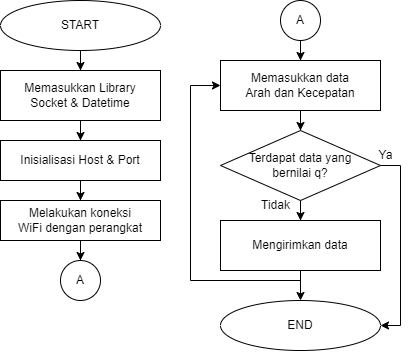
\includegraphics[scale=0.8]{gambar/10. Mengirim Data String WiFi.png}
  % Keterangan gambar yang diinputkan
  \caption{Flowchart Mengirim Data String Melalui WiFi \parencite{ekatama2024perancangan}}
  % Label referensi dari gambar yang diinputkan
  \label{fig:Flowchart Mengirim Data String Melalui WiFi}
\end{figure}


\subsection{Kontroller Kursi Roda}
Pada tahap ini, ESP32 akan mendapatkan arah hasil klasifikasi pose wajah dalam bentuk huruf A, B, C, D, atau E. Menurut penelitian yang telah dilakukan sebelumnya \parencite{ekatama2024perancangan}, proses ESP32 menerima data string dari NUC telah divisualisasikan pada flowchat Gambar \ref{fig:Flowchart Menerima Data String Melalui Access Point WiFi Pada ESP32}. Program ini dirancang sebagai server WiFi yang akan menerima data dari perangkat yang terhubung yang dalam pengujian kali ini adalah NUC. Jika server terhubung dengan \emph{client}, maka program akan memasuki fungsi if yang akan mengulang-ulang terus dan menunggu adanya data yang dikirimkan oleh \emph{client}. Data yang diterima akan dibaca secara terus-menerus dan akan dimasukkan kedalam variabel receivedData. Setelah itu, data yang diterima akan di-\emph{decode} menjadi bentuk string. Program akan terus berjalan dan menunggu adanya data yang dikirimkan oleh \emph{client}.

\begin{center}
  \centering
  % Nama dari file gambar yang diinputkan
  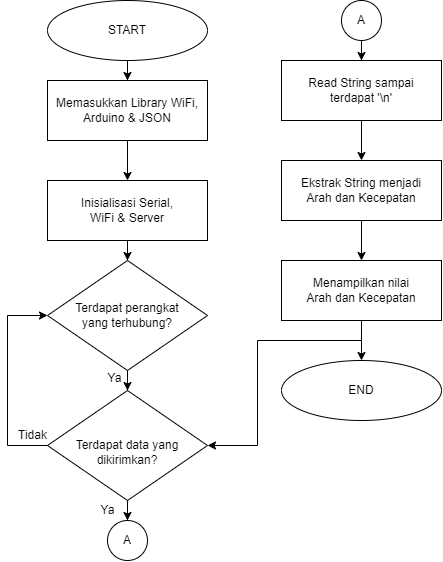
\includegraphics[width=0.8\textwidth]{gambar/4. Menerima String WiFi.png}
  % Keterangan gambar yang diinputkan
  \captionof{figure}{Flowchart Menerima Data String Melalui Access Point WiFi Pada ESP32 \parencite{ekatama2024perancangan}}
  % Label referensi dari gambar yang diinputkan
  \label{fig:Flowchart Menerima Data String Melalui Access Point WiFi Pada ESP32}
\end{center}


Berdasarkan penelitian yang telah dilakukan \parencite{ekatama2024perancangan}, telah dirancang sebuah kontroller motor kursi roda dengan skematik alatnya seperti yang tertera pada Gambar \ref{fig:skematikkontrol}. ESP32 akan terhubung dengan dua buah H-Bridge Motor Driver dan sebuah DC-DC Converter. Masing-masing H-Bridge Motor Driver akan terhubung ke motor roda kiri dan motor roda kanan agar dapat menggerakan roda kursi roda. DC-DC Converter akan terhubung ke baterai sebagai sumber daya. Kontroller ini akan mengontrol pergerakan motor kursi roda berdasarkan arah yang didapatkan dari hasil klasifikasi pose wajah. 

\begin{center}
  \centering
  % Nama dari file gambar yang diinputkan
  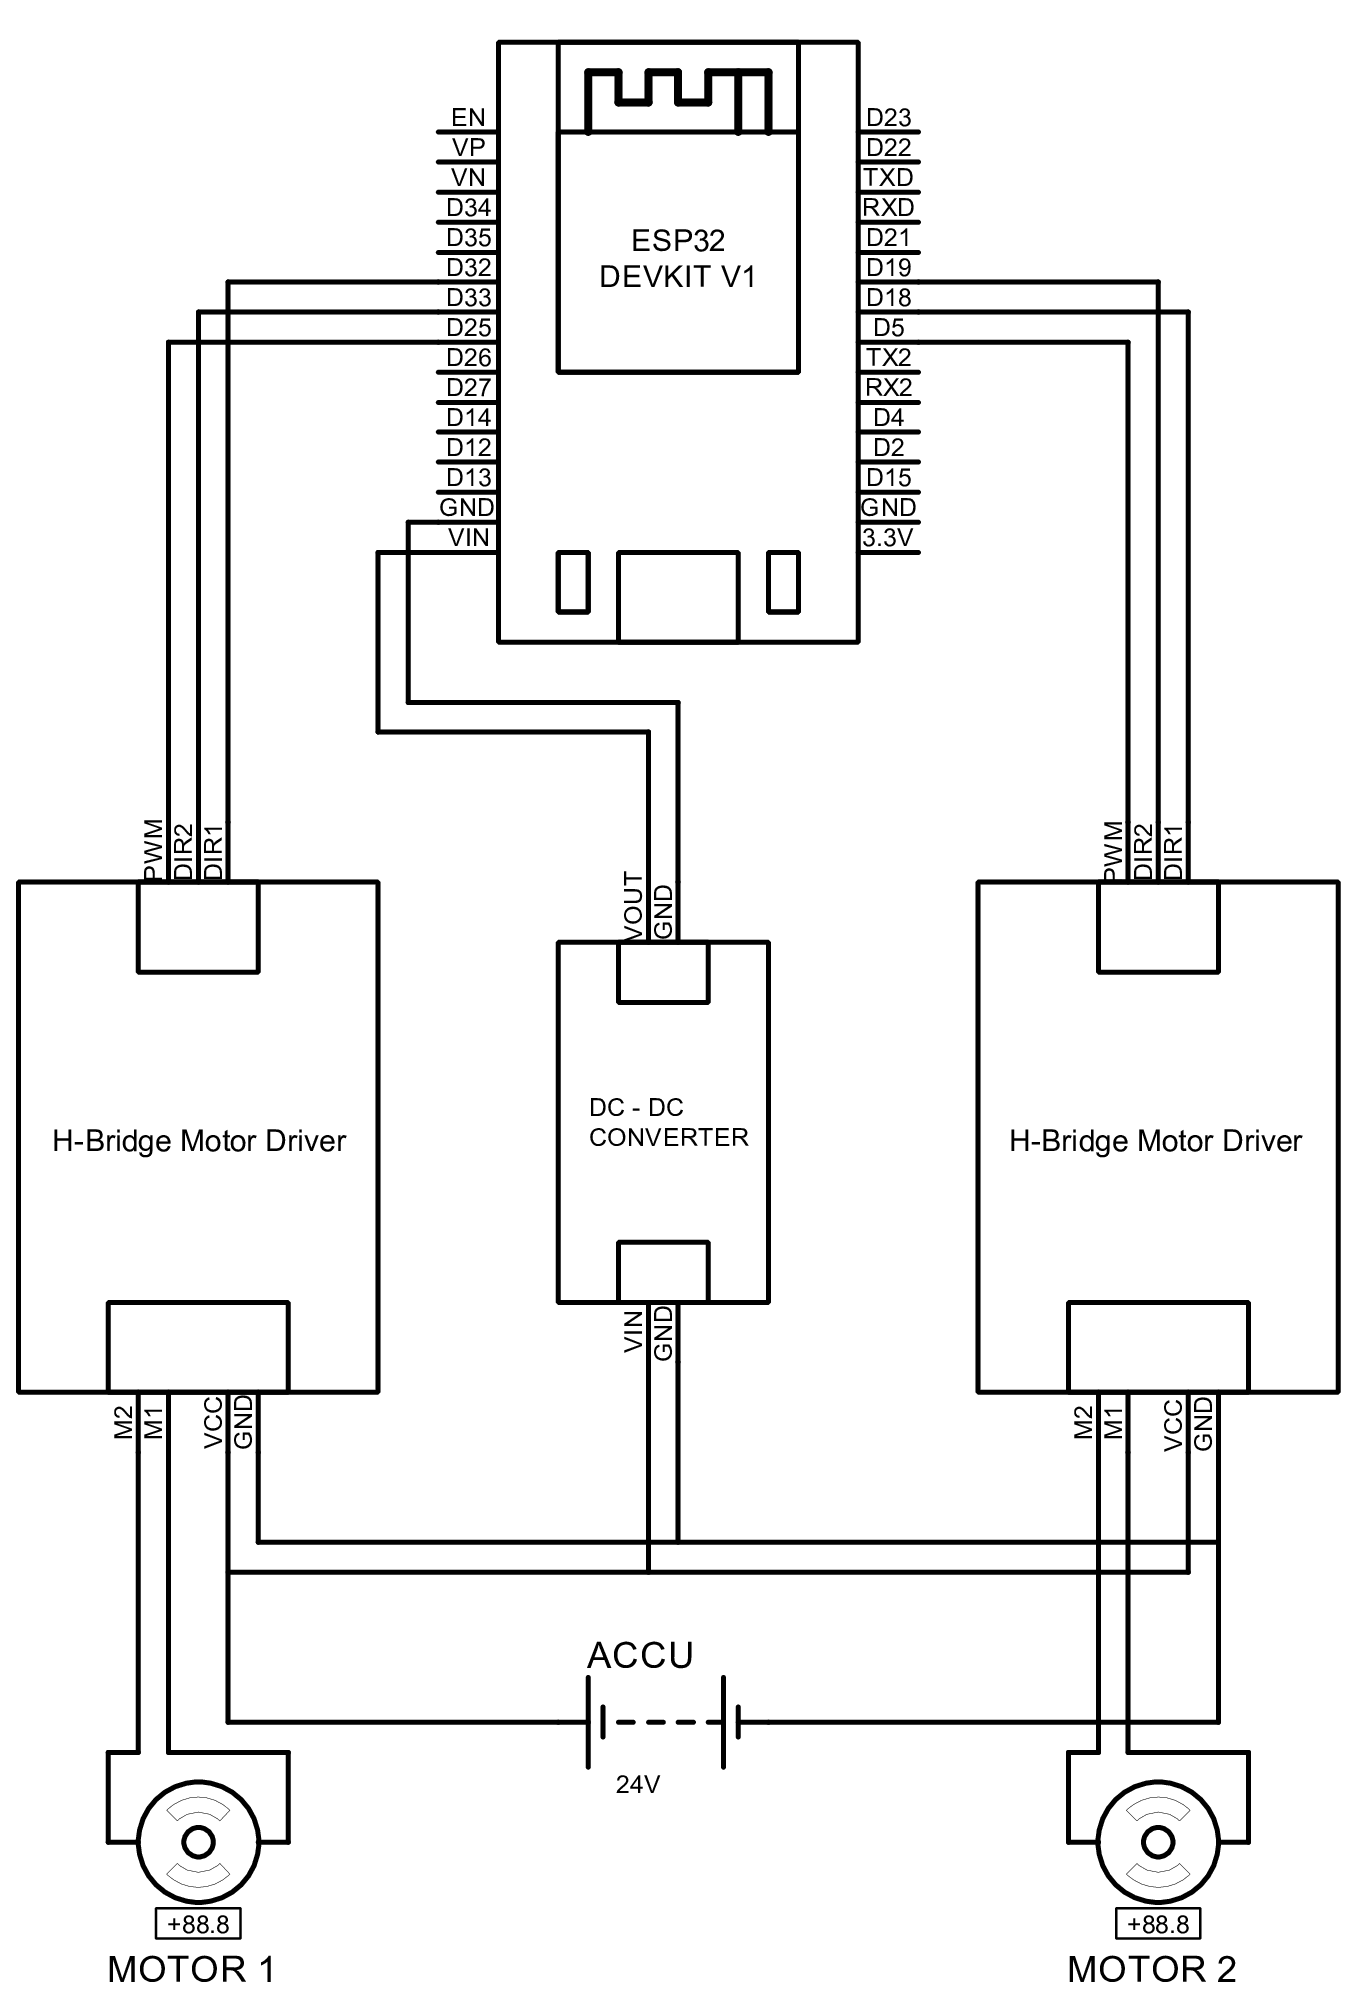
\includegraphics[width=0.7\textwidth]{gambar/Schematics.png}
  % Keterangan gambar yang diinputkan
  \captionof{figure}{Skematik \parencite{ekatama2024perancangan}}
  % Label referensi dari gambar yang diinputkan
  \label{fig:skematikkontrol}
\end{center}

Untuk proses kontrol motor kursi roda, telah direpresentasikan pada flowchart Gambar \ref{fig: Flowchart Kontrol Motor Kursi Roda Melalui Access Point WiFi} sesuai dengan penelitian yang telah dilakukan \parencite{ekatama2024perancangan}. Program ini dirancang untuk mengendalikan pergerakan motor DC dengan cara memproses perintah yang telah diterima melalui koneksi jaringan wifi. Untuk mengontrol pergerakan kursi roda, terdapat dua buah metode. Metode pertama adalah differential drive yang mana ketika kursi roda akan berbelok ke kanan, maka roda kanan akan bergerak mundur dan berbelok ke kiri sedangkan roda kirinya akan bergerak maju dan berbelok ke kanan. Ketika akan berbelok ke kiri, maka akan terjadi hal sebaliknya. Ketika akan bergerak maju atau mundur makan kedua roda akan bergerak secara bersamaan kearah yang diinginkan. Metode kedua adalah pergerakan biasa yang mana ketika kursi roda akan berbelok ke kanan, maka roda kanan akan diam sedangkan roda kirinya akan bergerak maju dan berbelok ke kanan. Ketika akan berbelok ke kiri, maka akan terjadi hal sebaliknya. Ketika akan bergerak maju atau mundur makan kedua roda akan bergerak secara bersamaan kearah yang diinginkan. Untuk penelitian kali ini akan digunakan metode kedua untuk menggerakan roda pada kursi roda.
\begin{figure}[H]
  \centering
  % Nama dari file gambar yang diinputkan
  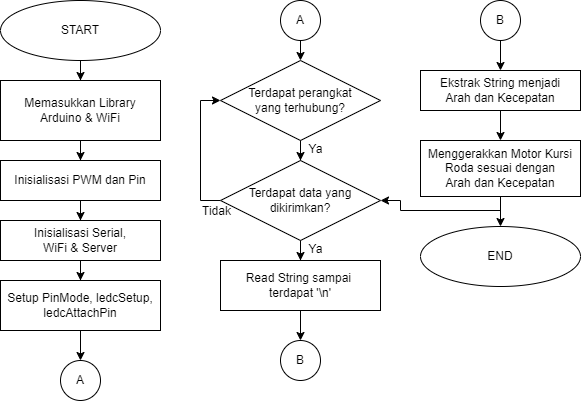
\includegraphics[scale=0.7]{gambar/8. Kontrol Motor WiFi.png}
  % Keterangan gambar yang diinputkan
  \caption{ Flowchart Kontrol Motor Kursi Roda Melalui Access Point WiFi \parencite{ekatama2024perancangan}}
  % Label referensi dari gambar yang diinputkan
  \label{fig: Flowchart Kontrol Motor Kursi Roda Melalui Access Point WiFi}
\end{figure}



\section{\emph{Software}}

\begin{center}
  \centering
  % Nama dari file gambar yang diinputkan
  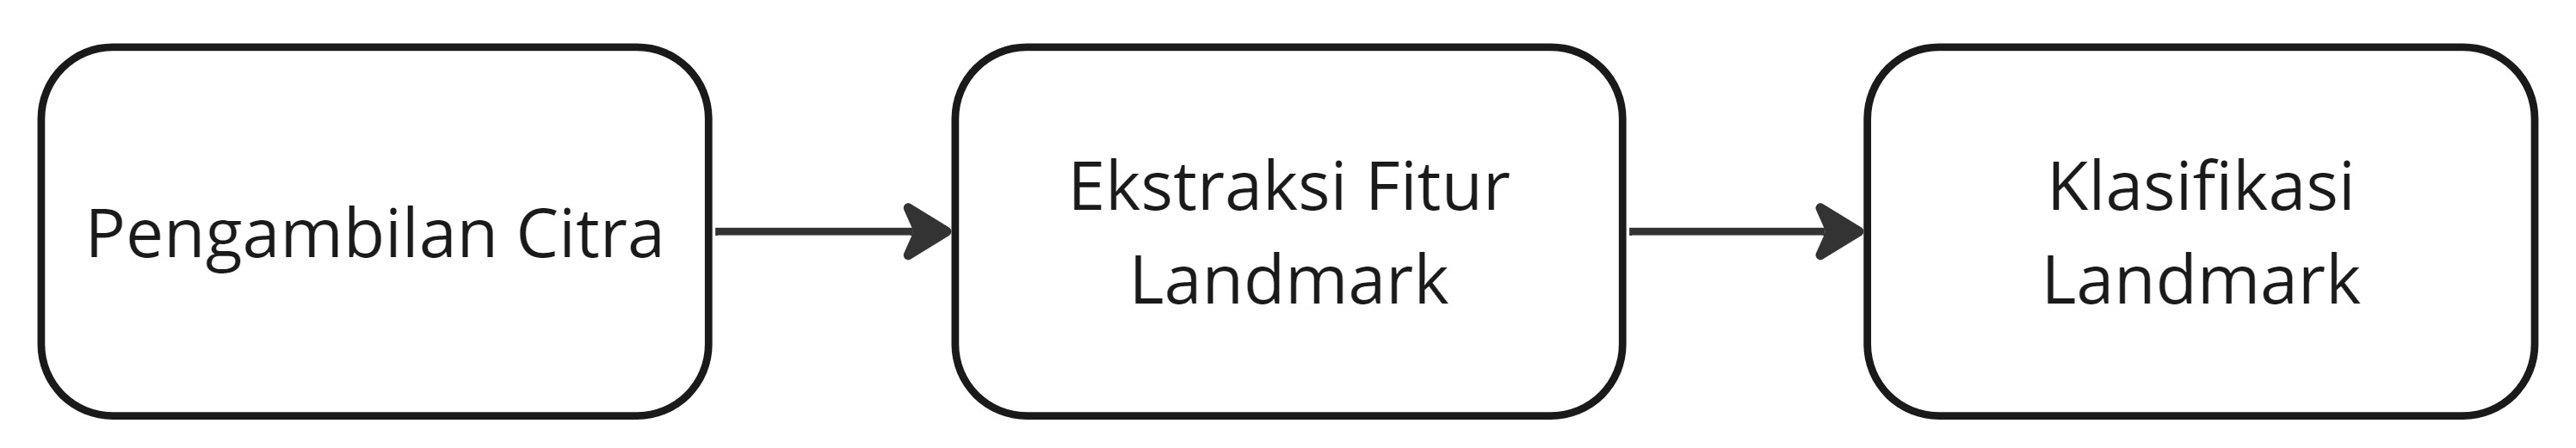
\includegraphics[width=0.9\textwidth]{gambar/blokdiagramsoftwareidpendek.jpg}
  % Keterangan gambar yang diinputkan
  \captionof{figure}{Blok diagram \emph{software}}
  % Label referensi dari gambar yang diinputkan
  \label{fig:Blok Diagram}
\end{center}

\subsection{Citra}
Data yang digunakan sebagai dataset adalah citra pose wajah yang diambil secara langsung dari seseorang. Data citra pose wajah diambil dengan cara menggunakan kamera webcam yang terhubung pada laptop dan kemudian setiap frame dari video tersebut akan dijadikan satu buah citra pose wajah. Kemudian, citra wajah yang telah didapat akan diproses apakah terdapat citra wajah atau tidak. Kemudian, akan dilakukan pendeteksian secara \emph{realtime} untuk mendeteksi ada tidaknya citra wajah. 

\subsection{Ekstraksi Fitur Landmark}

Setelah terdeteksi adanya wajah, mediapipe akan melakukan tracking dengan menggunakan \emph{pre-trained} model yang dimiliki dari mediapipe itu sendiri. Kemudian untuk setiap \emph{frame} yang terdeteksi akan diproses data gambarnya. Mediapipe akan mengidentifikasi \emph{Region of Interest} (ROI) dimana sekiranya terdapat fitur wajah. \emph{Pre-trained} model kemudian akan memprediksi koordinat titik-titik tertentu (landmark) pada ROI. Landmark yang didapat adalah dalam bentuk koordinat \emph{pixel}. Dilakukanlah normalisasi yang mengubah koordinat \emph{pixel} menjadi skala relatif berdasarkan dimensi frame yang telah dideteksi. Normalisasi ini dilakukan agar landmark tetap konsisten meskipun dalam ukuran frame dan resolusi yang berbeda. Selanjutnya, untuk meningkatkan akurasi dan independensi dataset, dibuatlah gambar yang hitam sepenuhnya. Hal ini akan mengisolasi landmark yang akan digambar dan membuatnya menjadi lebih mudah terdeteksi ketika melakukan training nantinya.

Kemudian, mediapipe menggambarkan fitur-fitur landmark wajah pada background hitam. Terdapat tiga jenis style landmark untuk wajah yang dapat dibuat oleh mediapipe, yaitu FACEMESH\textunderscore TESSELATION, FACEMESH\textunderscore CONTOURS, dan FACEMESH\textunderscore IRISES. Pada FACEMESH\textunderscore TESSELATION, landmark digambarkan dengan sejumlah segitiga yang membentuk permukaan wajah. Setiap segitiga yang digambar menghubungkan tiga buah titik landmark pada wajah. Sementara itu, FACEMESH\textunderscore CONTOURS, landmark yang digambarkan hanya merepresentasikan kontur atau garis luar dari wajah tanpa menggambarkan permukaan wajah secara detail. Di sisi lain, FACEMESH\textunderscore IRISES, landmark yang digambar hanya pada iris mata saja. Pada penelitian kali ini akan digunakan FACEMESH\textunderscore TESSELATION karena landmark yang digambar lebih detail dan kompleks sehingga akan meningkatkan akurasi pendeteksian pose wajah. Pada dokumentasi Mediapipe mengenai face landmark,telah disebutkan bahwa pada landmark wajah terdapat titik-titik yang berjumlah 468 yang diperkirakan dalam ruang 3D secara real-time. Akan tetapi, pada penelitian kali ini hanya menggunakan landmark 2D yang memungkinkan representasi wajah menjadi invarian terhadap skala. 

\subsection{Klasifikasi Landmark}
Untuk dapat melakukan pengklasifikasian, diperlukan sebuah model yang merupakan hasil \emph{training} dari \emph{Convolutional Neural Network} (CNN). Model yang didapat dari hasil \emph{training} akan melakukan pengklasifikasian secara \emph{real-time} setiap kali wajah terdeteksi. Model CNN yang digunakan pada penelitian kali ini memiliki lima kelas yang akan merepresentasikan arah gerak kursi roda. Kelima kelas tersebut adalah kanan yang direpresentasikan dengan wajah menghadap kanan, kiri yang direpresentasikan dengan wajah menghadap kiri, maju yang direpresentasikan dengan wajah menghadap atas, mundur yang direpresentasikan dengan wajah menghadap bawah, dan \emph{stop} yang direpresentasikan dengan wajah menghadap depan. Pada Gambar \ref{fig:contohcitrawajah} dapat dilihat contoh data citra wajah yang digunakan untuk tiap-tiap kelasnya.

\begin{figure}[H]
  \centering
  \begin{subfigure}{0.3\textwidth}
      \centering
      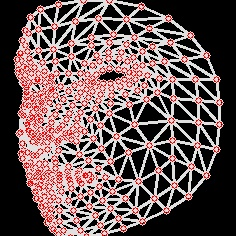
\includegraphics[width=\linewidth]{gambar/normal kanan.jpg}
      \caption{Citra kelas kanan}
      \label{fig:image1}
  \end{subfigure}
  \hfill
  \begin{subfigure}{0.3\textwidth}
      \centering
      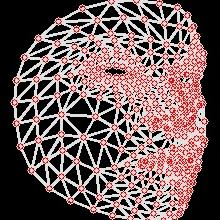
\includegraphics[width=\linewidth]{gambar/normal kiri.jpg}
      \caption{Citra kelas kiri}
      \label{fig:image2}
  \end{subfigure}
  \hfill
  \begin{subfigure}{0.3\textwidth}
      \centering
      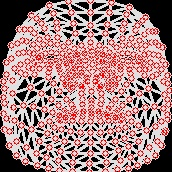
\includegraphics[width=\linewidth]{gambar/normal maju.jpg}
      \caption{Citra kelas maju}
      \label{fig:image3}
  \end{subfigure}
  
  \begin{subfigure}{0.3\textwidth}
      \centering
      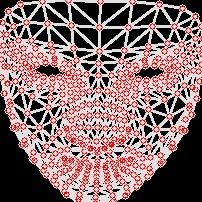
\includegraphics[width=\linewidth]{gambar/normal mundur.jpg}
      \caption{Citra kelas mundur}
      \label{fig:image4}
  \end{subfigure}
  \hfill
  \begin{subfigure}{0.3\textwidth}
      \centering
      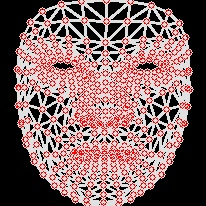
\includegraphics[width=\linewidth]{gambar/normal stop.jpg}
      \caption{Citra kelas \emph{stop}}
      \label{fig:image5}
  \end{subfigure}
  \caption{Contoh citra wajah}
  \label{fig:contohcitrawajah}
\end{figure}


Terdapat 2 model dengan arsitektur berbeda pada penelitian kali ini. Arsitektur CNN yang digunakan untuk mendapatkan pertama model pada penelitian kali ini memiliki 7 \emph{layer}. Layer pertama adalah Convolutional 2D layer yang melakukan 64 filter dengan ukuran kernel (3,3) pada input dengan dimensi 140 x 140 pixels dan 3 /emph{color channels}. Fungsi utama layer ini adalah untuk mengekstraksi fitur-fitur dari gambar yang diinputkan dengan cara menggeser filter melintasi gambar yang mana akan membantu dalam melakukan pendeteksian tepi, warna, gradien, dan lain-lain. Setiap filter akan menghasilkan map fitur yang merepresentasikan fitur-fitur yang ada pada gambar input. Layer ini juga merupakan layer inputnya. Selanjutnya layer kedua adalah \emph{hidden layer} yang pertama yang berupa Max Pooling 2D dengan \emph{pool size} (2,2). Layer ini akan mengurangi dimensi spasial pada map fitur dengan cara mengambil nilai maksimum yang ada pada \emph{pool} 2 x 2. Hal ini akan mengurangi kompleksitas komputasi dengan mengecilkan map fitur dan membantu membuat pendeteksian menjadi invarian terhadap skala dan orientasi. Layer ketiga adalah \emph{hidden layer} kedua yang merupakan Convolutional 2D dengan 256 filter, \emph{kernel size} (3,3), dan ReLU sebagai fungsi aktivasinya. Layer tersebut akan melakukan pemrosesan lebih lanjut terhadap map fitur yang telah didapatkan dari layer sebelumnya, sehingga dapat mengenali pola yang lebih rumit seperti tekstur dan bentuk. Layer keempat adalah Max Pooling 2D dengan \emph{pool size} (2,2) yang akan terus mengecilkan ukuran map fitur, sehingga dapat meringkas semua fitur-fitur yang telah didapatkan dengan data yang lebih sedikit. Layer kelima adaah Flatten yang menjadikan output dari layer sebelumnya menjadi array satu dimensi atau menjadi satu vektor yang panjang. Layer ini berfungsi sebagai jembatan antara convolutional layer dengan dense layer karena dense layer memerlukan data 1D. Layer selanjutnya atau layer keenam adalah Dense atau \emph{fully connected} layer pertama yang memiliki 512 unit dan menggunakan ReLU sebagai fungsi aktivasinya. Layer ini akan mengambil fitur-fitur yang sudah di-\emph{flatten} dan kemudian mempelajari kombinasi fitur yang non-linear. Layer terakhir atau ketujuh yang digunakan adalah dense atau \emph{fully connected} layer kedua yang memiliki jumlah unit yang sama dengan jumlah kelas yang akan diprediksi, yaitu 5. Layer ini juga merupakan layer output. Arsitektur CNN untuk model pertama divisualisasikan pada Gambar \ref{fig:Arsitektur CNN Model 1}. Untuk model kedua, memiliki arsitektur yang mirip dengan model pertama akan tetapi terdapat sedikit perbedaan pada jumlah filter dan jumlah unit pada dense layer. Model kedua memiliki 64 filter pada layer pertama, 128 unit pada layer ketiga, dan 256 unit pada dense layer pertama. Arsitektur CNN untuk model kedua divisualisasikan pada Gambar \ref{fig:Arsitektur CNN Model 2}.


\begin{figure}[H]
  \centering
  % Nama dari file gambar yang diinputkan
  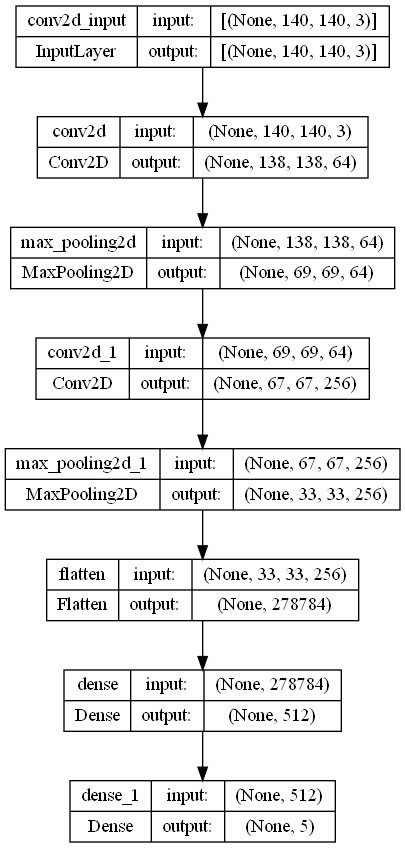
\includegraphics[scale=0.6]{gambar/tabelcnn.png}
  % Keterangan gambar yang diinputkan
  \caption{Arsitektur CNN Model 1}
  % Label referensi dari gambar yang diinputkan
  \label{fig:Arsitektur CNN Model 1}
\end{figure}

\begin{figure}[H]
  \centering
  % Nama dari file gambar yang diinputkan
  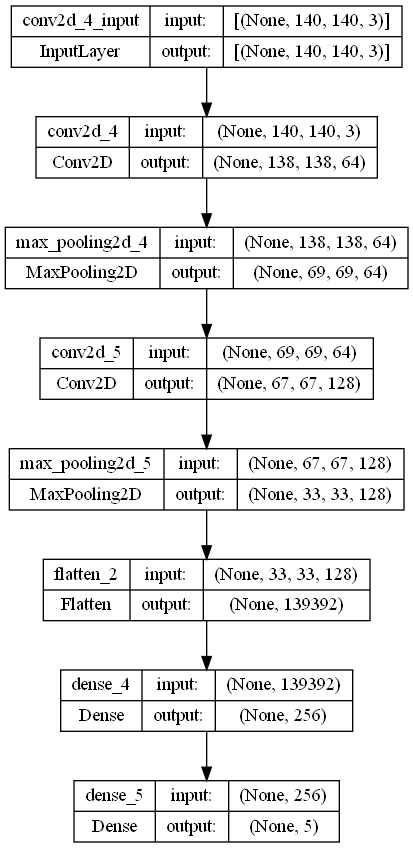
\includegraphics[scale=0.6]{gambar/tabelcnntdk.png}
  % Keterangan gambar yang diinputkan
  \caption{Arsitektur CNN Model 2}
  % Label referensi dari gambar yang diinputkan
  \label{fig:Arsitektur CNN Model 2}
\end{figure}



Pada gambar \ref{fig:arsitekturcnngambar}, setiap jenis layer direpresentasikandengan warna-warna yang berbeda. Warna kuning pada layer merepresentasikan Convolutional Layer, warna merah merepresentasikan layer Max Pooling, warna hijau merepresentasikan layer \emph{flatten}, dan warna biru merepresentasikan layer \emph{dense}.
\begin{figure}[H]
  \centering
  % Nama dari file gambar yang diinputkan
  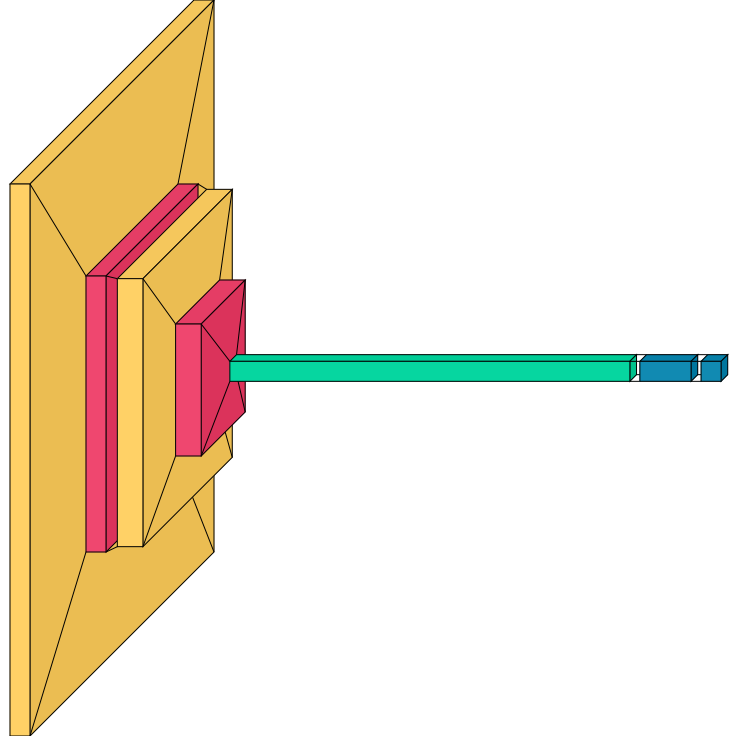
\includegraphics[scale=0.4]{gambar/arsitekturcnngambar.png}
  % Keterangan gambar yang diinputkan
  \caption{Diagram Arsitektur CNN Model 1}
  % Label referensi dari gambar yang diinputkan
  \label{fig:arsitekturcnngambar}
\end{figure}

\begin{figure}[H]
  \centering
  % Nama dari file gambar yang diinputkan
  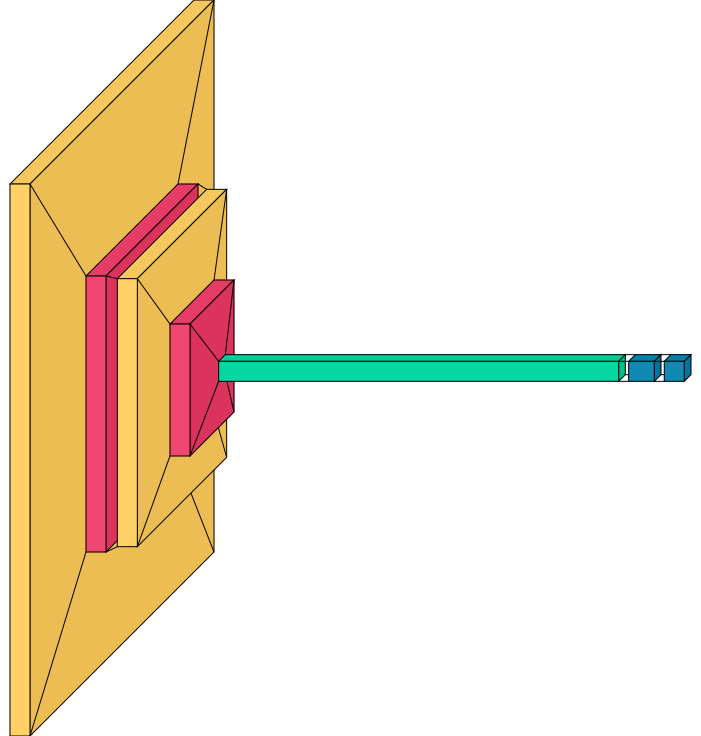
\includegraphics[scale=0.4]{gambar/arsitekturcnngambartdk.png}
  % Keterangan gambar yang diinputkan
  \caption{Diagram Arsitektur CNN Model 2}
  % Label referensi dari gambar yang diinputkan
  \label{fig:arsitekturcnngambar}
\end{figure}


Sistem kontrol yang digunakan untuk menggerakkan kursi roda terbagi menjadi lima kelas arah yang memiliki indeks dan direpresentasikan dengan menggunakan huruf. Hal ini dilakukan karena perbedaan antara cara kerja Python dan Arduino IDE. Indeks ini digunakan pada saat penghitungan pada proses klasifikasi. Ketika citra wajah diklasifikasikan, citra wajah tersebut akan dicocokkan ke indeks. Jika tidak cocok, maka indeks akan dilanjutkan dari 0 ke 1, 1 ke 2 sampai data citranya cocok barulah diklasifikasikan kepada kelas yang direpresentasikan oleh indeks tersebut.

\begin{table}[H]
\begin{longtable}{|c|c|c|}
  \caption{Kelas yang Digunakan}
  \label{tb:EnergiKecepatan}                                   \\
  \hline
  \rowcolor[HTML]{C0C0C0}
  \textbf{Index Kelas} & \textbf{Index Arah} & \textbf{Hasil Klasifikasi} \\
  \hline
  0   & E   & Kanan   \\
  1   & A   & Kiri   \\
  2   & B    & Maju   \\
  3   & D   & Mundur   \\
  4   & C    & Stop   \\
    \hline
\end{longtable}
\end{table}
